%rubber: module pdflatex

\documentclass[11pt,a4paper]{article}

\usepackage{sdp_doc} % SDP style file
\usepackage[english]{babel}


%%%%%%%%% START OF USER SETTINGS %%%%%%%%%%%%%%%%%%
\title{DELIVERY PLATFORM}
% Enter here some information needed to fill in the template Title to appear
% on the front pages (will be filled in via the \sdpfrontpage command)
\newcommand{\bigdoctitle}{Delivery Platform\xspace}
% Title to go in the "Document Status Sheet" Document number
\newcommand{\docnr}{SKA-TEL-SDP-00000??\xspace}
% Context
\newcommand{\context}{(SDP Work Package)}
% Revision
\newcommand{\revision}{1.0\xspace}
% Author(s)
\newcommand{\docauthor}{A.\ Bcdefg, H.\ Ijklm\xspace}
% Lead author (goes in the footer)
\newcommand{\leadauthor}{A.\ Bcdefg\xspace}
% Release date (YYYY-MM-DD)
\newcommand{\docudate}{2015-02-06\xspace}
% Document classification
\newcommand{\classification}{Unrestricted}
% Status of the document (draft/final/etc.)
\newcommand{\docstatus}{Draft\xspace}

% The definitions below are used for the signature tables in the preamble of
% the document
\newcommand{\firstsigname}{Name 1 - to be filled in}
\newcommand{\firstsigdesignation}{Designation 1 - to be filled in}
\newcommand{\firstsigaffiliation}{Affiliation 1 - to be filled in}

\newcommand{\secondsigname}{Name 2 - to be filled in}
\newcommand{\secondsigdesignation}{Designation 2 - to be filled in}
\newcommand{\secondsigaffiliation}{Affiliation 2 - to be filled in}

% Table with version numbers
\newcommand{\versiontable}{
  \begin{tabularx}{\textwidth}{|X|X|X|X|}
    \hline
    \bf{Version} & {\bf Date of issue} & {\bf Prepared by} & {\bf Comments}\\
    \hline
    1.0 & & & \\
    \hline
  \end{tabularx}
}

%%%%%%%%%%%%% END OF USER SETTINGS %%%%%%%%%%%%%%%%%%%

% Table with signatures
\newcommand{\signaturetable}[3]{
  \begin{tabularx}{\textwidth}{|X|X|X|}
    \hline
    Name & Designation & Affiliation\\
    \hline
    {#1} & {#2} & {#3}\\
    \hline
    Signature \& Date: & & \\
    & & \\
    & & \\
    \hline
  \end{tabularx}
}


% Table with affiliations
\newcommand{\organisationtable}{
  \begin{center}
    \sffamily{\bf ORGANISATION DETAILS}\end{center}
  \begin{table}[htbp]
    \centering
    \begin{tabular}[htbp]{|l|l|}
      \hline
      Name & Science Data Processor Consortium\\
      \hline
    \end{tabular}
  \end{table}
}


%%%%%%%%%%%%%%%%%%%% START YOUR DOCUMENT HERE %%%%%%%%%%%%%%%%%

\begin{document}

% load automatic pages
\sdpfrontpage

\sdptableofcontents

% Add here the abbreviations used in your document
\sdplistofabbreviations
\begin{basedescript}{\desclabelstyle{\pushlabel}\desclabelwidth{6em}}
    \item[SOMETHING] Something \vspace{-0.2cm}
    \item[OTHER] Other something \vspace{-0.2cm}
    \item[OTHER] Other other something \vspace{-0.2cm}
\end{basedescript} 

% Add here the symbols used in your document
\sdplistofsymbols
\begin{basedescript}{\desclabelstyle{\pushlabel}\desclabelwidth{6em}}
    \item[$N_\mathrm{something}$] Number of somethings \vspace{-0.2cm}
    \item[OTHER] Other something \vspace{-0.2cm}
    \item[OTHER] Other other something \vspace{-0.2cm}
\end{basedescript} 


\sdplistoffigures

\sdplistoftables

% Add here the executive summary
\sdpsummary

% Add to the table the list of applicable and reference documents
% (this is NOT meant for your usual bibiliography, only for SKA docs)
\sdpreferencedocs

\subsection*{Applicable Documents}

The following documents are applicable to the extent stated herein. In the
event of conflict between the contents of the applicable documents and this
document, \emph{the applicable documents} shall take precedence.

\begin{center}{
\begin{tabularx}{\textwidth}{|X|X|}
    \hline
    \bf{Reference} & \bf{Reference}\\
    \bf{Number} & \\
    \hline
\end{tabularx}}
\end{center}

\subsection*{Reference Documents}

The following documents are referenced in this document. In the event of
conflict between the contents of the referenced documents and this document,
\emph{this document} shall take precedence.

\begin{center}{
\begin{tabularx}{\textwidth}{|X|X|}
    \hline
    \bf{Reference} & \bf{Reference}\\
    \bf{Number} & \\
    \hline
\end{tabularx}}
\end{center}




% The actual content goes here
\newpage
\section{Introduction}

A little example sentence.

\clearpage
\section{Functional Description}
\label{section:main}

This is the operational context for the Data Delivery Platform.

\begin{figure}[h]
  \centering
  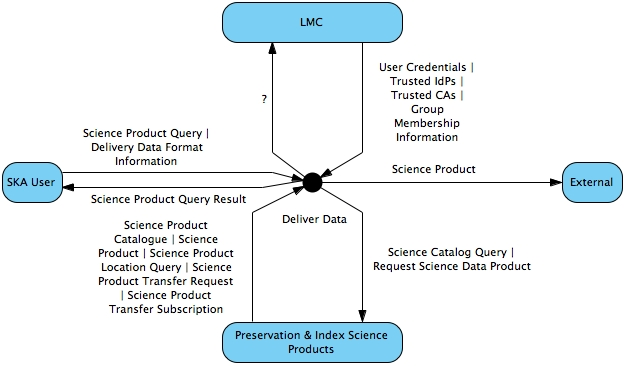
\includegraphics[width=0.95\textwidth]{L0.jpg}
  \caption{Data Delivery Context.}
\end{figure}

\subsection{Data Delivery Function Decomposition}

\begin{figure}[h]
  \centering
  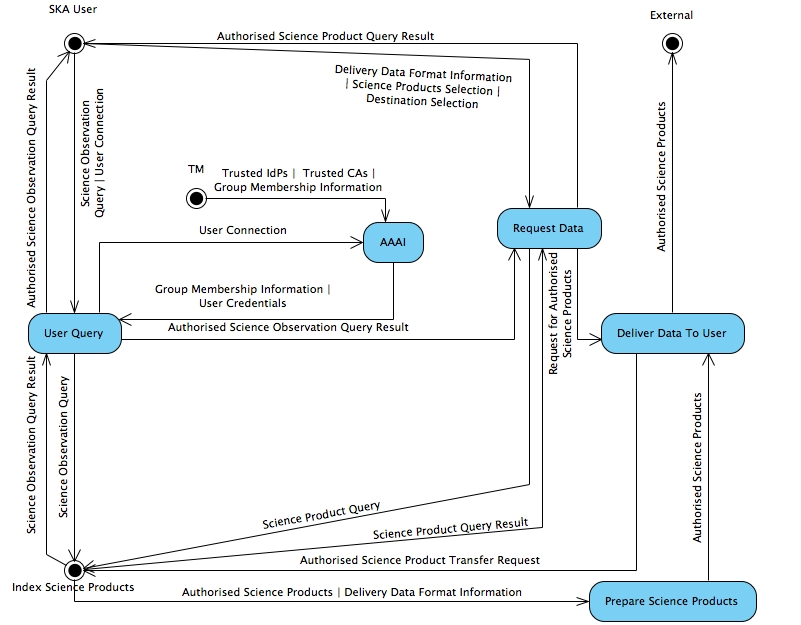
\includegraphics[width=0.85\textwidth]{L1.jpg}
  \caption{Data Delivery Function Decomposition.}
\end{figure}

And some text. But why isn't the figure above this line in the source document, above this line in the preview?


\subsubsection{AAAI}

Description of AAAI decomposition here.

\subsubsection{Query And Request}

\begin{figure}[h]
  \centering
  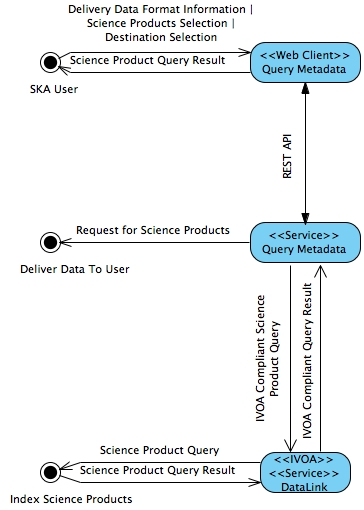
\includegraphics[width=0.45\textwidth]{l2.jpg}
  \caption{Query and Request Function Decomposition.}
\end{figure}

Description of Query and Request decomposition here.

\subsubsection{Prepare and Deliver}

Description of Prepare and Deliver decomposition here.

\clearpage
\section{Conclusions}
\label{section:conclusions}

And here also.


%  Add the bibliography
\clearpage
\addcontentsline{toc}{section}{References}
\bibliography{your_bibfile}%


\end{document}

%%% Local Variables: 
%%% mode: latex
%%% TeX-master: t
%%% End: 
